\documentclass[10pt,a4paper]{article}

\usepackage{a4wide}
\setlength{\parskip}{0.5ex plus0.1ex minus0.1ex}
\setlength{\parindent}{0em}

\usepackage[round,longnamesfirst]{natbib}
\usepackage{hyperref}

\newcommand{\strong}[1]{{\normalfont\fontseries{b}\selectfont #1}}
\newcommand{\class}[1]{\textsf{#1}}
\newcommand{\code}[1]{\texttt{#1}}
\newcommand{\pkg}[1]{\strong{#1}}
\newcommand{\samp}[1]{`\texttt{#1}'}
\newcommand{\proglang}[1]{\textsf{#1}}

\usepackage{Sweave}
%% \VignetteIndexEntry{Data structures for association rules}


\begin{document}
%% ------------------------------------------------------------------
%% ------------------------------------------------------------------
\title{A Computational Environment for Mining Association Rules and
  Frequent Item Sets}
\author{Michael Hahsler and Bettina Gr{\"u}n and Kurt Hornik}
\maketitle
\sloppy
%% ------------------------------------------------------------------
%% ------------------------------------------------------------------
\begin{abstract}
  Mining frequent itemsets and association rules is a popular and well
  researched approach for discovering interesting relationships between
  variables in large databases.  The \proglang{R} package \pkg{arules}
  presented in this paper provides a basic infrastructure for creating
  and manipulating input data sets and for analyzing the resulting
  itemsets and rules.  The package also includes interfaces to two fast
  mining algorithms, the popular \proglang{C} implementations of Apriori
  and Eclat by Christian Borgelt.  These algorithms can be used to mine
  frequent itemsets, maximal frequent itemsets, closed frequent itemsets
  and association rules.
\end{abstract}

%% ------------------------------------------------------------------
%% ------------------------------------------------------------------

\section{Introduction}

Mining frequent itemsets and association rules is a popular and well
researched method for discovering interesting relations between
variables in large databases. \cite{arules:Piatetsky-Shapiro:1991}
describes analyzing and presenting strong rules discovered in databases
using different measures of interest.  Based on the concept of strong
rules, \cite{arules:Agrawal+Imielinski+Swami:1993} introduced the
problem of mining association rules from transaction data as follows.

Let $I=\{i_1, i_2,\ldots,i_n\}$ be a set of $n$ binary attributes called
\emph{items}.  Let $\mathcal{D} = \{t_1, t_2, \ldots, t_m\}$ be a set of
transactions called the \emph{database}.  Each transaction
in~$\mathcal{D}$ contains a subset of the items in~$I$.

A \emph{rule} is defined as an implication of the form $X \Rightarrow Y$
where $X, Y \subseteq I$ and $X \cap Y = \emptyset$.  The sets of items
(for short \emph{itemsets}) $X$ and $Y$ are called \emph{antecedent}
(left-hand-side or LHS) and \emph{consequent} (right-hand-side or RHS)
of the rule.

To select interesting rules from the set of all possible rules,
constraints on various measures of significance and interest can be
used.  The best-known constraints are minimum thresholds on support and
confidence.  \emph{Support} is defined on an itemset as the proportion
of transactions in the data set which contain the itemset.  All itemsets
which have a support above a set minimum support threshold are called
\emph{frequent itemsets}.  
Finding frequent itemsets can be seen as a simplification of
the unsupervised learning problem called
``mode finding'' or 
``bump hunting''~\citep{arules:Hastie+Tibshirani+Friedman:2001}.
For these problems each item is seen as a variable.
The goal is to find
prototype values so that the probability density
evaluated at these values is sufficiently large.
However, for practical applications with a large number of variables, 
probability estimation will be unreliable and computationally too expensive.
This is why in practice frequent itemsets are used instead of 
probability estimation.

\emph{Confidence} is defined on rules as $\mathrm{conf}(X\Rightarrow Y)
= \mathrm{supp}(X \cup Y) / \mathrm{supp}(X)$.  This can be interpreted
as an estimate of the probability $P(Y|X)$, the probability of finding
the RHS of the rule in transactions under the condition that these
transactions also contain the LHS 
\citep[see e.g.,][]{arules:Hipp+Guentzer+Nakhaeizadeh:2000}.  
Association rules are
required to satisfy both constraints, minimum support and
minimum confidence, at the same time.

At medium to low support values, often a great number of frequent
itemsets are found in a database.  However, since the definition of
support enforces that all subsets of a frequent itemset have to be also
frequent, it is sufficient to only mine all \emph{maximal frequent
  itemsets}, defined as frequent itemsets which are not proper subsets
of any other frequent
itemset~\citep{arules:Zaki+Parthasarathy+Ogihara+Li:1997}.  Another
approach to reduce the number of mined itemsets is to only mine
\emph{frequent closed itemsets.}  An itemset is closed if no proper
superset of the itemset is contained in each transaction in which the
itemset is contained~\citep{arules:Pasquier+Bastide+Taouil+Lakhal:1999,
  arules:Zaki:2004}.  Frequent closed itemsets are a superset of the
maximal frequent itemsets.  Their advantage over maximal frequent
itemsets is that in addition to be able to infer all frequent itemsets,
they also preserve the support information for all frequent itemsets
which can be important for computing additional interest measures after
the mining process is finished (e.g., confidence for rules
generated from the found itemsets, or 
\emph{all-confidence}~\citep{arules:Omiecinski:2003}).


A practical solution to the problem of finding too many 
association rules with support and confidence is
to further filter or rank found rules using additional interest measures.
A popular measure for this purpose is 
\emph{lift}~\citep{arules:Brin+Motwani+Ullman+Tsur:1997}.
Lift is defined on rules as $\mathrm{lift}(X \Rightarrow Y) = 
\frac{\mathrm{supp}(X \cup Y)}{ \mathrm{supp}(X) \mathrm{supp}(Y)}$.
It can be interpreted as the deviation of the support of the whole 
rule from the support expected under independence given the 
supports of the LHS and the RHS.
Greater lift values indicate stronger associations.


In the last decade research on algorithms to solve the frequent itemset
problem has been abundant.  \cite{arules:Goethals+Zaki:2004} compare the
currently fastest algorithms.  Among these algorithms are the
implementations of the Apriori and Eclat algorithms by
\cite{arules:Borgelt:2003} interfaced in the package \pkg{arules}.
The two algorithms use very different mining strategies.  Apriori,
developed by \cite{arules:Agrawal+Srikant:1994}, is a level-wise,
breadth-first algorithm which counts transactions.  In contrast, Eclat
\citep{arules:Zaki+Parthasarathy+Ogihara+Li:1997} employs equivalence
classes, depth-first search and set intersection instead of counting.
The algorithms can be used to mine frequent itemsets, maximal frequent
itemsets and closed frequent itemsets.  The implementation of Apriori
can additionally be used to generate association rules.

The \proglang{R} package \pkg{arules} presented in this paper provides
the infrastructure needed to create and manipulate input data sets for
the mining algorithms and for analyzing the resulting itemsets and
rules.  Since it is common to work with large sets of rules and
itemsets, the package uses sparse matrix representation to minimize
memory usage.  The infrastructure provided by the package was also
created to explicitly facilitate easy extensions, both for interfacing
new algorithms and for adding new types of interest measures and
associations.

The rest of the paper is organized as follows: In the next section, we
give an overview of the data structure implemented in the package
\pkg{arules}.  In Sections~\ref{sec:transactions} and
\ref{sec:associations} we introduce the functionality of the classes to
handle transaction data and associations.  In
Section~\ref{sec:interfaces} we describe the way mining algorithms are
interfaced in \pkg{arules} using the already implemented interfaces for
Apriori and Eclat as examples.  We provide several examples in
Sections~\ref{sec:example-screen} to \ref{sec:example-allconf}.  The
first two examples show typical \proglang{R} sessions for preparing, 
analyzing and
manipulating a transaction data set, and for mining association rules.
The third example demonstrates how \pkg{arules} can be extended to
integrate a new interest measure.  We conclude with a summary of the
features and advantage of the package \pkg{arules} as a computational
environment for mining association rules and frequent itemsets.

%% ------------------------------------------------------------------
%% ------------------------------------------------------------------
\section{Data structure overview\label{sec:overview}}

To enable the user to represent and work with input and output data of
association rule mining algorithms in \proglang{R}, a well thought out
structure is necessary which can deal in an efficient way with large
amounts of sparse binary data.  The \proglang{S4} class structure 
implemented in
the package \pkg{arules} is presented in
figure~\ref{fig:arules-classes}.

\begin{figure}[tp]
\centering
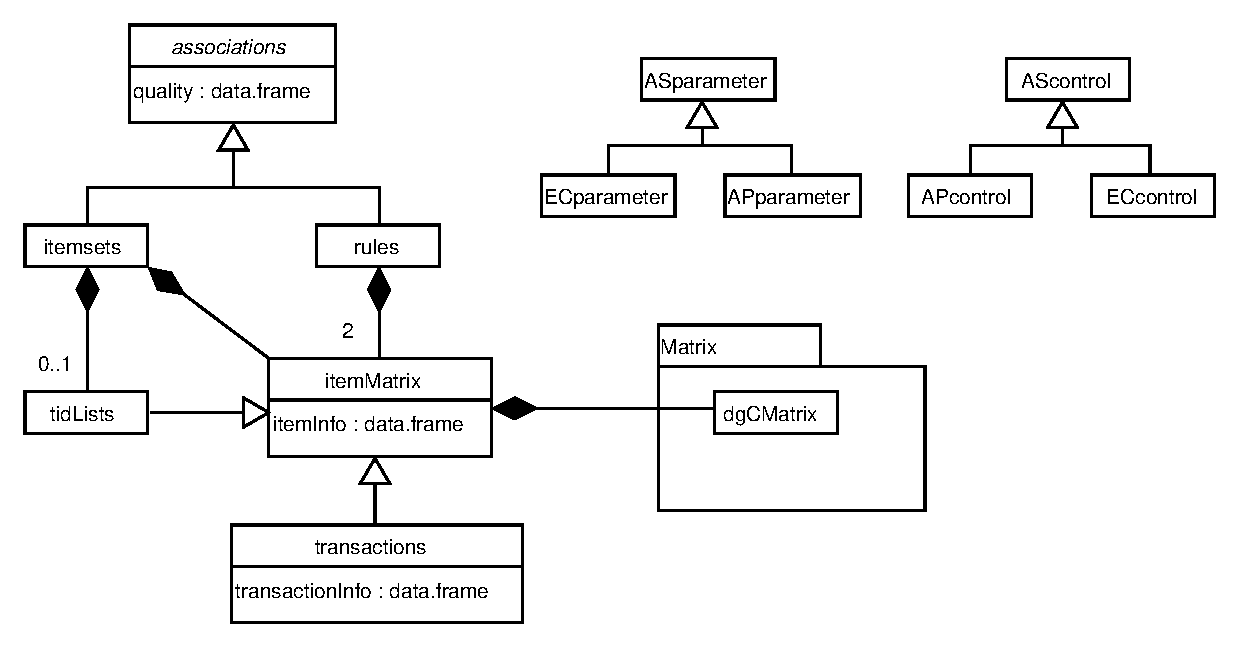
\includegraphics[width=14cm]{arules-classes}
\caption{UML class diagram of the \pkg{arules}
package.\label{fig:arules-classes}}
\end{figure}

For input data the class \class{transactions} is provided.
The output of the mining algorithms comprises the classes
\class{itemsets} and \class{rules} representing a set of itemsets or
a set of rules, respectively.
Both classes directly extend
a common virtual class called \class{associations} which provides a
common interface.
In this structure it is easy to add a new type of associations by adding
a new class that extends \class{associations}.

Items in \class{associations} and \class{transactions} are implemented
by the \class{itemMatrix} class which provides a facade for the sparse
matrix implementation \class{dgCMatrix} from package \pkg{Matrix}
\citep{arules:Bates+Maechler:2005}.
Objects of the \class{itemMatrix} class are not intended to be directly
accessed by the end user of \pkg{arules}.  The interfaces of
\class{associations} and \class{transactions} can be used without
knowledge of how the internal representation of the data works.
However, the data structure in \class{itemMatrix} or even the
\class{dgCMatrix} can be directly accessed if necessary (e.g., to
efficiently compute a distance matrix between itemsets for clustering).

To control the behavior of the mining algorithms, the two classes
\class{ASparameter} and \class{AScontrol} are used.  Since each
algorithm can use additional algorithm-specific parameters, we
implemented for each interfaced algorithm its own set of control
classes.  We used the prefix \class{AP} for Apriori and \class{EC} for
Eclat.  In this way, it is easy to extend the control classes when
interfacing a new algorithm.

%% ------------------------------------------------------------------
%% ------------------------------------------------------------------

\section{Transaction data\label{sec:transactions}}

The main application of association rules is for market basket analysis
where large transaction data sets are mined.  In this setting each
transaction contains the items which were purchased at one visit to a
retail store \citep[see e.g.,][]{arules:Berry+Linoff:1997}.
Transaction data are normally recorded by point-of-sale
scanners and consists of tuples of the form:

\begin{displaymath}
<\emph{transaction ID}, \emph{item ID}, \ldots >
\end{displaymath}

All tuples with the same transaction ID form a single transaction which
contains all the items given by the item IDs in the tuples.  Additional
information denoted by the dots might be available.  For example, the
customer ID might be available via a loyalty program in a supermarket.
Further information on transactions (e.g., time, location), on the items
(e.g., category, price) or on the customer (socio-demographic variables
as age, gender, etc.)  might be available.

For mining, the transaction data is first transformed into a binary
purchase incidence matrix with columns equal to the number of different
items and rows equal to the number of different transactions.  The
matrix entries represent the presence (1) or absence (0) of an item in a
particular transaction.  An example of a binary incidence matrix is
depicted in Figure~\ref{fig:incidenceMatrix}.
This format is often called the \emph{horizontal} database 
layout~\citep{arules:Zaki:2000}.
Alternatively, transaction data can be represented in a
\emph{vertical} database
layout in the form of \emph{transaction ID lists}~\citep{arules:Zaki:2000}.
In this format for each item a list of IDs of the
transactions the item is contained in is stored.
Depending on the algorithm, one of the layouts is used for mining.
In \pkg{arules} both layouts are implemented as the
classes~\class{transactions} and \class{tidLists} and the data can be
directly transformed from one format to the other.


\begin{figure}[tp]
\centering
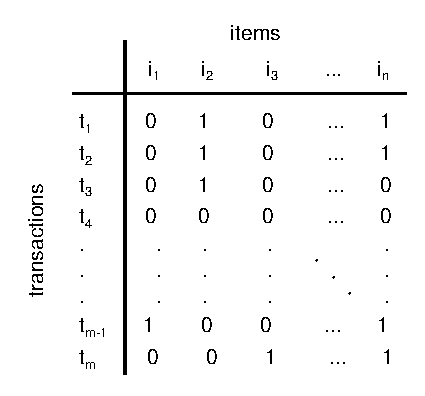
\includegraphics[width=5cm]{incidenceMatrix}
\caption{Example of a transaction data set represented as a binary incidence matrix.\label{fig:incidenceMatrix}}
\end{figure}


Since a typical supermarket transaction only contains a small number of
items compared to the total number of available items, the
binary incidence matrix will
in general be very sparse with many items and a very large number of
transactions.  A natural representation for such data is a sparse matrix
format.  For our implementation we chose the \class{dgCMatrix} which is
defined in the \proglang{R} package \pkg{Matrix} 
implemented by~\cite{arules:Bates+Maechler:2005}. The \class{dgCMatrix}
is a compressed, sparse, column-oriented matrix which contains the
indices of the rows unequal to zero, the pointers to the initial indices
of elements in each column and the non-zero elements of the matrix.
Since the package \pkg{Matrix} does not provide subset selection
functionality for \class{dgCMatrix}, we implemented a suitable function
in \proglang{C} and interfaced it as the subset selection method (\code{[}).
Despite the column orientation of the \class{dgCMatrix}, it is more
convenient to work with incidence matrices which are row-oriented.  This
makes the most important manipulation, selecting a set of transactions
from a data set for mining, more comfortable and efficient.  Therefore,
we implemented the class \class{itemMatrix} providing a row-oriented
facade to the \class{dgCMatrix} which stores a transposed incidence
matrix.  At this level also the constraint that the incidence matrix is
binary (and not real valued as the \class{dgCMatrix}) is enforced.
Additionally, \class{itemMatrix} stores item labels (e.g., name
of the items) and handles the necessary mapping between the item label and the
corresponding column number in the incidence matrix.  Optionally,
\class{itemMatrix} can also store additional information on items. For
example, the category hierarchy in a supermarket setting can be stored which
enables the analyst to select only transactions (or as we later see also rules
and itemsets) which contain items from a certain category (e.g., all dairy
products). 

For \class{itemMatrix}, basic methods including \code{dim}, subset
selection (\code{[}) and coercion from and to \class{matrix} and
\class{list} primitives are provided.  Additionally, methods specific to
the needs for \pkg{arules} are implemented. Since \class{itemMatrix} is
used to store a set of transactions or, more general, a set of itemsets,
we implemented a \code{length} method which returns the number of
elements in the set (i.e., the number of transactions or the number of
itemsets in the set).  Technically, \code{length} returns the number of
rows of the sparse matrix.  The \code{size} method returns a vector with
the sizes of each element in the set (row in the matrix).  For example,
for a purchase incidence matrix we will get a vector of length of the
number of transactions in the matrix and each element of the vector
contains the size (number of items) of the corresponding transaction.
This information can be used to select or filter unusually long or short
transactions.  Finally, an \code{image} method can be used to produce a
level plot of the binary matrix useful for quick visual inspection.  For
transaction data sets (e.g., point-of-sale data) a plot can be very
helpful for checking if the data set contains structural changes (e.g.,
items were not offered or out-of-stock during part of the observation
period) or to find abnormal transactions (e.g., transactions which
contain almost all items may point to recording problems).  Spotting
such problems can be very helpful for data preparation.

The class \class{transactions} directly extends \class{itemMatrix}
and inherits its basic matrix functionality (e.g., subset selection).
In addition, \class{transactions} has 
a slot to store additional information for each
transaction in form of a \class{data.frame}.
The slot can hold arbitrary named vectors with length equal to the
number of stored transactions.
In \pkg{arules} the slot is currently used to store transaction IDs,
however, it can easily be used to store user IDs, revenue or profit,
or other information on each transaction.
With this information subsets of transactions
(e.g., only transactions of a certain user or exceeding a set profit)
can be selected.
Objects of class \class{transactions} can be easily 
created by coercion from \class{matrix} or \class{list}.
If names are available in these data structures,
they are used as item labels or transaction IDs accordingly. 
To import data from a file, the \code{read.transactions} function is
provided. This function 
reads files structured as shown above and also the
very common format with 
one line per transaction
and the items separated by a predefined character.
Finally, the method \code{inspect} can be used to 
inspect transactions (e.g., an interesting transaction selected
with subset selection).

Another important application of mining association rules has been proposed by
\cite{arules:Piatetsky-Shapiro:1991} and \cite{arules:Srikant+Agrawal:1996} for
discovering interesting relationships between the values of categorical and
quantitative (metric) attributes.  For mining associations rules, non-binary
attributes have to be mapped to binary attributes. The straight forward mapping
method is to transform the metric attributes into $k$ ordinal attributes by
building categories (e.g., an attribute income might be transformed into a
ordinal attribute with the three categories: ``low'', ``medium'' and ``high'').
Then, in a second step, each categorical attribute with $k$ categories is
represented by $k$ binary dummy attributes which correspond to the items used
for mining.  An example application using questionnaire data can be found in
\cite{arules:Hastie+Tibshirani+Friedman:2001}.

The typical representation for data with categorical and quantitative
attributes in \proglang{R} is a \class{data.frame}.  First, a domain expert has
to create useful categories for all metric attributes.  This task is
supported in \proglang{R} by functions as \code{cut(x, \ldots)}, etc.  The
second step, the generation of binary dummy items, is automated in package
\pkg{arules} by the \code{coerce} method from \class{data.frame} to
\class{transactions}.  In this process, the original attribute names and
categories are preserved as additional item information and can be used
to select itemsets or rules which contain items referring to a certain original
attributes.  The resulting \class{transactions} object can be mined and
analyzed the same way as market basket data, see the example in
Section~\ref{sec:example-screen}.





%% ------------------------------------------------------------------
%% ------------------------------------------------------------------
\section{Sets of itemsets and sets of rules\label{sec:associations}}

The result of mining transaction data in \pkg{arules} are
\class{associations.} 
Conceptually, associations are sets of 
objects. Each object describes the relationship between some items (e.g., 
an itemset or a rule) and
has values for different measures of quality assigned.
Such quality measures can be measures of significance (e.g., support) 
or measures of interest (e.g., confidence, lift)
or other measures (e.g., revenue covered by the association).

All association types have a common interface suitable for set operations.
Methods for subset extraction (\code{[} and the \code{subset} method), 
getting the number of elements in the set with \code{length}, 
and sorting the set using the values of different quality measures 
(method \code{SORT}) are available.
A \code{summary} method produces a short overview of the set
and with \code{inspect} individual associations can be inspected.


In \pkg{arules} currently
sets of itemsets (e.g., used for frequent itemsets of their 
closed or maximal subset) and
sets of rules (e.g., association rules) are implemented as associations.  
Both itemsets and rules directly extend the
virtual class \class{associations}.
Class \class{itemsets} contains one \class{itemMatrix} object to store
the items as a binary matrix where each row in the matrix represents an
itemset. In addition, it may contain
transaction ID lists as an object of class \class{tidLists} 
which is implemented as a
sparse matrix (reusing \class{itemMatrix}).  
When representing transactions, \class{tidLists}
stores for each item a transaciton list. Here
it stores for each itemset a list of transaction IDs in which the itemset
appears. Such lists are currently only returned by \code{eclat}.
Class \class{rules} consists of two \class{itemMatrix} objects
representing the left-hand-side (LHS) and the right-hand-side (RHS) of
the rules, respectively.  

The items in the associations and the
quality measures can be accessed
and manipulated in a safe way using accessor and replace methods for
\code{quality}, \code{items}, \code{lhs} and \code{rhs}.  In addition
the association classes have built-in validity checking which ensures
that all elements have a matching dimension.

It is simple to add new quality measures to existing associations.
Since the \code{quality} slot holds a \class{data.frame}, additional
columns with new quality measures can be added.  These new measures can
then be used to sort or select associations using the \code{SORT} or the
\code{subset} methods.  Adding a new type of associations to
\pkg{arules} is easy as well.  One has only to implement a new class
extending the virtual \class{associations} class.

%% ------------------------------------------------------------------
%% ------------------------------------------------------------------

\section{Mining algorithm interfaces\label{sec:interfaces}}

In package \pkg{arules} we interface free reference implementations of
Apriori and Eclat by Christian Borgelt
\citep{arules:Borgelt+Kruse:2002,arules:Borgelt:2003}.  The code is
called directly from \proglang{R} by the functions \code{apriori} and
\code{eclat} and the data objects are directly passed from \proglang{R} to
the \proglang{C} code and back without writing to external files.
The implementations can mine association rules, frequent itemsets,
and closed and maximal frequent itemsets. 


%% <<apriori>>=
%% library(arules)
%% args(apriori)
%% args(eclat)
%% @

The input format of the data for the \code{apriori} and
\code{eclat} functions is
\class{transactions} or a data format which can be coerced to
\class{transactions} (e.g., \class{matrix} or \class{list}).
The algorithm parameters are divided into two groups represented
by the arguments \code{parameter} and \code{control}.
The mining parameters (\code{parameter}) change the
characteristics of the mined itemsets or rules  (e.g., the
minimum support) and the control parameters (\code{control})
influence the
performance of the algorithm (e.g., an initial sorting of the items
with respect to their frequency).
These arguments have to be instances of the
classes \class{APparameter} and \class{APcontrol} for
the function \code{apriori}
or \class{ECparameter} and \class{ECcontrol} for
the function \code{eclat}, respectively.  Alternatively, data which can be coerced to
these classes (e.g., \code{NULL}
which will give the default values or a named list
with names equal to slot names to change the default values) can be passed.
In these classes, each slot specifies a different parameter and the values.  The
default values are equal to the defaults of the stand-alone \proglang{C}
programs \citep{arules:Borgelt:2004} except that by
default the more common original
support definition (instead of the
support of only the antecedent)
is used for the specified minimum support required.

For \code{apriori} the appearance feature implemented by Christian
Borgelt can also be used.  With argument \code{appearance} of function
\code{apriori} one can specify which items have to or cannot appear in
itemsets or rules.  For more information on this feature we refer to the
Apriori manual~\citep{arules:Borgelt:2004}.

The output of the functions \code{apriori} and \code{eclat} is an object
of a class extending \class{associations} which contains the sets of mined
associations and can be further analyzed using the methods provided for
these classes.

It is straightforward to interface additional algorithms which use an
incidence matrix or transaction ID list representation as input.  The
necessary steps are:

\begin{enumerate}
 \item Adding interface code to the algorithm, preferably by directly
  calling into the native implementation language (rather than using
  files for communication), and an \proglang{R} function calling this
  interface.
 \item Implementing extensions for \class{parameter} and
  \class{control}.
\end{enumerate}

There exist many different algorithms which solve the frequent 
and closed frequent itemset problems.
Each algorithm has specific strengths which can be important for
very large databases.
Such algorithms, e.g. kDCI, LCM, FP-Growth or Patricia, are
discussed in~\cite{arules:Goethals+Zaki:2003}.  
The source code is available on the internet and can be interfaced 
in the future for \pkg{arules}. 


%% ------------------------------------------------------------------
%% ------------------------------------------------------------------


\section{Example 1: Analyzing and preparing a data set \label{sec:example-screen}}

In this example, 
we show how a data set can be analyzed and manipulated
before associations are mined.
This is important for finding problems in the data set which 
could make the mined associations useless or at least inferior
to associations mined on a properly prepared data set.
For the example,
we look at the \code{Epub} transaction data contained in
package \pkg{arules}.  This data set contains downloads of documents
from the Electronic Publication platform of the Vienna University of
Economics and Business Administration available via
\url{http://epub.wu-wien.ac.at} from January 2003 to April 2005.

First, we load \pkg{arules} and the data set.

\begin{Schunk}
\begin{Sinput}
> library("arules")
\end{Sinput}
\begin{Soutput}
Loading required package: stats4
Loading required package: Matrix
\end{Soutput}
\begin{Sinput}
> data("Epub")
> Epub
\end{Sinput}
\begin{Soutput}
transactions in sparse format with
 2771 transactions (rows) and
 419 items (columns)
\end{Soutput}
\end{Schunk}

We see that the data set consists of 2771 transactions
and is represented as a sparse matrix with 2771 rows
and 419 columns which represent the items. 
Next, we use the summary method to get more information about the 
data set.

\begin{Schunk}
\begin{Sinput}
> summary(Epub)
\end{Sinput}
\begin{Soutput}
transactions as itemMatrix in sparse format with
 2771 rows (elements/itemsets/transactions) and
 419 columns (items)

most frequent items:
epub-wu-01_11d epub-wu-01_4c6 epub-wu-01_2cd  epub-wu-01_71 epub-wu-01_364 
           177            100             90             90             89 
       (Other) 
          4436 

element (itemset/transaction) length distribution:
   1    2    3    4    5    6    7    8    9   10   11   12   13   14   15   16 
1976  411  164   78   43   20   13   12   10    5    7    4    4    2    1    3 
  17   18   19   20   22   24   25   28   34   38   74 
   2    2    5    2    1    1    1    1    1    1    1 

   Min. 1st Qu.  Median    Mean 3rd Qu.    Max. 
  1.000   1.000   1.000   1.798   2.000  74.000 

includes extended transaction information - examples:
                     transactionIDs           TimeStamp
1 epub-wu-01_session4795-1041447099 2003-01-01 19:59:00
2 epub-wu-01_session4797-1041486295 2003-01-02 06:46:01
3 epub-wu-01_session479a-1041497371 2003-01-02 09:50:38
\end{Soutput}
\end{Schunk}

The summary method displays the most frequent items in the data set,
information about the transaction length distribution and that the data
set contains some extended transaction information.  We see that the
data set contains transaction IDs and in addition time stamps (using class
\class{POSIXct}) for the
transactions.  The additional information can be used for analyzing the
data set.

\begin{Schunk}
\begin{Sinput}
> year <- strftime(as.POSIXlt(transactionInfo(Epub)[["TimeStamp"]]), 
+     "%Y")
> table(year)
\end{Sinput}
\begin{Soutput}
year
2003 2004 2005 
 988 1375  408 

\end{Soutput}
\end{Schunk}

We selected only the year part of the time stamps. For 2003, the first year
in the data set we have 988 transactions.
We can select the corresponding transactions and inspect the structure
using a level-plot. 

\begin{Schunk}
\begin{Sinput}
> Epub_2003 <- Epub[year == "2003"]
> length(Epub_2003)
\end{Sinput}
\begin{Soutput}
[1] 988
\end{Soutput}
\begin{Sinput}
> image(Epub_2003)
\end{Sinput}
\end{Schunk}
\begin{center}
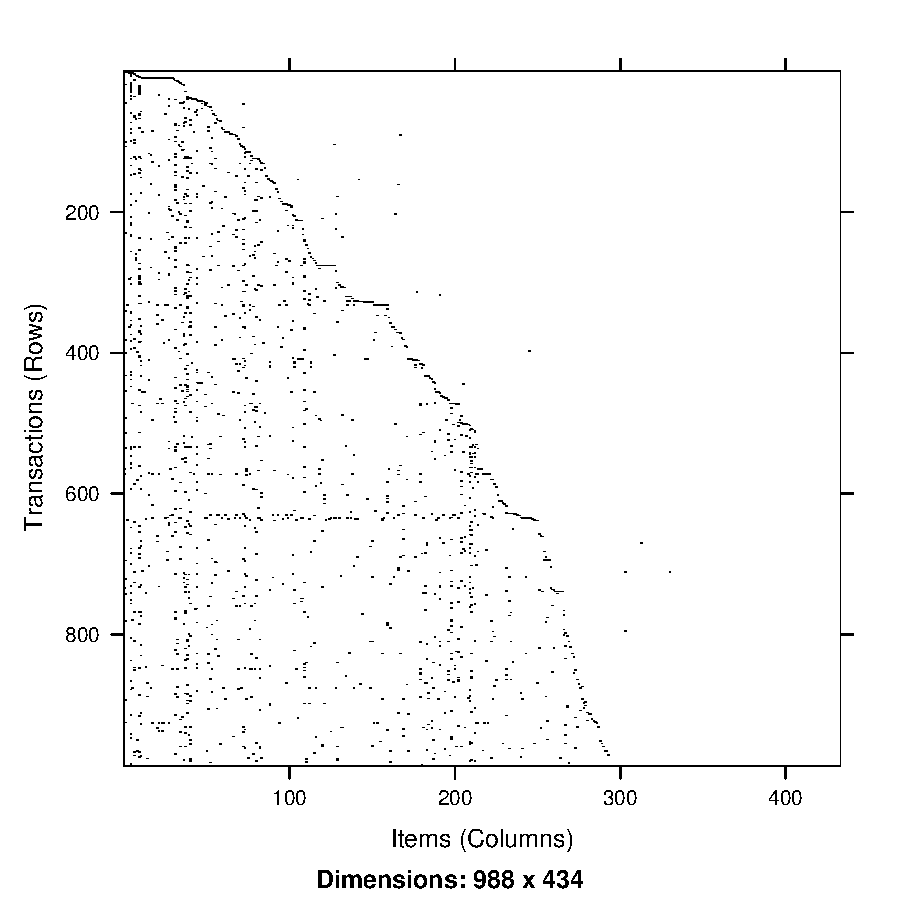
\includegraphics[width=8cm]{arules-epub_image}
\end{center}

The plot is a direct visualization of the binary incidence matrix where
the the dark dots represent the ones in the matrix.  From the plot we
see that the items in the data set are not evenly distributed.  In fact,
the white area to the top right side suggests, that in the beginning of
2003 only very few items were available (less than 50) and then during
the year more items were added until it reached a number of around 300
items. Also, we can see that there are two transactions in the data set
which contain a very high number of items (denser horizontal lines).
These transactions need further investigation since they could originate
from data collection problems (e.g., a web robot downloading many
documents from the publication site).  To find the very long
transactions we can use the size method and select very long
transactions (containing more than 20 items).

\begin{Schunk}
\begin{Sinput}
> transactionInfo(Epub_2003[size(Epub_2003) > 20])
\end{Sinput}
\begin{Soutput}
                       transactionIDs           TimeStamp
301 epub-wu-01_session56e2-1051611211 2003-04-29 12:30:38
580 epub-wu-01_session6308-1061133365 2003-08-17 17:16:12
896 epub-wu-01_session72dc-1072722731 2003-12-29 19:35:35

\end{Soutput}
\end{Schunk}

We found three long transactions and printed the corresponding
transaction information. Of course, size can also be used in a similar
fashion to remove long or short transactions.

Transactions can be inspected using the inspect method. 
Since the long transactions identified above would result in
a very long printout, we will inspect 
the first 5 transactions in the subset for 2003.

\begin{Schunk}
\begin{Sinput}
> inspect(Epub_2003[1:5])
\end{Sinput}
\begin{Soutput}
  items                               transactionIDs           TimeStamp
1 {epub-wu-01_154} epub-wu-01_session4795-1041447099 2003-01-01 19:59:00
2 {epub-wu-01_3d6} epub-wu-01_session4797-1041486295 2003-01-02 06:46:01
3 {epub-wu-01_16f} epub-wu-01_session479a-1041497371 2003-01-02 09:50:38
4 {epub-wu-01_f4,                                                       
   epub-wu-01_11d,                                                      
   epub-wu-01_1a7} epub-wu-01_session47b7-1041526514 2003-01-02 17:55:50
5 {epub-wu-01_83}  epub-wu-01_session47bb-1041535625 2003-01-02 20:27:44

\end{Soutput}
\end{Schunk}

Most transactions contain one item. Only transaction 4 contains three items. 
For further inspection transactions can be converted into a list with:

\begin{Schunk}
\begin{Sinput}
> as(Epub_2003[1:5], "list")
\end{Sinput}
\begin{Soutput}
$"epub-wu-01_session4795-1041447099"
[1] "epub-wu-01_154"

$"epub-wu-01_session4797-1041486295"
[1] "epub-wu-01_3d6"

$"epub-wu-01_session479a-1041497371"
[1] "epub-wu-01_16f"

$"epub-wu-01_session47b7-1041526514"
[1] "epub-wu-01_f4"  "epub-wu-01_11d" "epub-wu-01_1a7"

$"epub-wu-01_session47bb-1041535625"
[1] "epub-wu-01_83"


\end{Soutput}
\end{Schunk}

Finally, transaction data in horizontal layout can be converted to
transaction ID list in vertical layout using coercion.

\begin{Schunk}
\begin{Sinput}
> Epub_tidLists <- as(Epub, "tidLists")
> Epub_tidLists
\end{Sinput}
\begin{Soutput}
tidLists in sparse format for
 419 items/itemsets (rows) and
 2771 transactions (columns)

\end{Soutput}
\end{Schunk}

For performance reasons the transaction ID list
is also stored in a sparse matrix. To get a list, coercion to \class{list}
can be used.

\begin{Schunk}
\begin{Sinput}
> as(Epub_tidLists[1:3], "list")
\end{Sinput}
\begin{Soutput}
$"epub-wu-01_154"
[1] "epub-wu-01_session4795-1041447099" "epub-wu-01_session6082-1058883924"
[3] "epub-wu-01_session60dd-1059130239" "epub-wu-01_session67db-1065044430"
[5] "epub-wu-01_session769c-1075191357" "epub-wu-01_session7ee3-1079450030"

$"epub-wu-01_3d6"
 [1] "epub-wu-01_session4797-1041486295" "epub-wu-01_session4893-1042136277"
 [3] "epub-wu-01_session48f4-1042453749" "epub-wu-01_session4ca3-1044889013"
 [5] "epub-wu-01_session52c6-1049273642" "epub-wu-01_session5712-1051701668"
 [7] "epub-wu-01_session58e3-1052992410" "epub-wu-01_session5984-1053467491"
 [9] "epub-wu-01_session5b20-1054675502" "epub-wu-01_session5c20-1055421043"
[11] "epub-wu-01_session5dc0-1056639134" "epub-wu-01_session5eac-1057261298"
[13] "epub-wu-01_session6599-1063473887" "epub-wu-01_session673d-1064583856"
[15] "epub-wu-01_session683e-1065381126" "epub-wu-01_session6f2f-1069854482"
[17] "epub-wu-01_session708a-1070754608" "epub-wu-01_session7a0c-1076882429"
[19] "epub-wu-01_session7de5-1078926808" "epub-wu-01_session89db-1084827080"
[21] "epub-wu-01_session9227-1089148583" "epub-wu-01_session9941-1094031566"
[23] "epub-wu-01_sessiona4d7-1100508833" "epub-wu-01_sessiona8c0-1102612273"
[25] "wu01_session4450a-1045050224"      "wu01_session4a129-1057762457"     
[27] "wu01_session4d25a-1066490150"     

$"epub-wu-01_16f"
[1] "epub-wu-01_session479a-1041497371" "epub-wu-01_session56e2-1051611211"
[3] "epub-wu-01_session630c-1061175093" "epub-wu-01_session72dc-1072722731"
[5] "epub-wu-01_session8b3e-1085510896" "epub-wu-01_session91ab-1088878266"
[7] "epub-wu-01_sessiona202-1098976943" "epub-wu-01_sessiona7b9-1101827029"


\end{Soutput}
\end{Schunk}

In this representation each item has an entry
which is a vector of all transactions it occurs in.
Transaction ID list can be directly used as input for mining algorithms which 
use such a vertical database layout to mine associations.


\section{Example 2: Preparing and mining a 
questionnaire data set\label{sec:example-adult}}

As a second example, 
we prepare and mine questionnaire data.
We use the Adult data set from the UCI machine
learning repository \citep{arules:Blake+Merz:1998} provided by
package~\pkg{arules}.  This data set is similar to the data used by
\cite{arules:Hastie+Tibshirani+Friedman:2001}.  The data originates from
the U.S. census bureau database and contains 48842 instances with 14
attributes like age, work class, education, etc. 
In the original applications of the data, the
attributes were used to predict the income level of individuals.
We added the attribute income with levels \code{Low} and \code{High},
representing an income of $\le \$50,000$ and $> \$50,000$, respectively.
This data is included in \pkg{arules} 
as the data set \code{Adult}.


\begin{Schunk}
\begin{Sinput}
> library("arules")
> data("Adult")
> dim(Adult)
\end{Sinput}
\begin{Soutput}
[1] 48842    15
\end{Soutput}
\begin{Sinput}
> Adult[1:2, ]
\end{Sinput}
\begin{Soutput}
  age        workclass fnlwgt education education-num     marital-status
1  39        State-gov  77516 Bachelors            13      Never-married
2  50 Self-emp-not-inc  83311 Bachelors            13 Married-civ-spouse
       occupation  relationship  race  sex capital-gain capital-loss
1    Adm-clerical Not-in-family White Male         2174            0
2 Exec-managerial       Husband White Male            0            0
  hours-per-week native-country income
1             40  United-States  small
2             13  United-States  small
\end{Soutput}
\end{Schunk}


\code{Adult} contains a mixture of categorical and metric attributes and
needs some preparations before it can be transformed into
transaction data suitable for association mining.
First, we remove the two attributes \code{fnlwgt} and
\code{education-num}. The first attribute is a weight calculated
by the creators of the data set from control data provided by
the Population Division of the U.S. census bureau. 
The second removed attribute is just a numeric representation of the
attribute \code{education} which is also part of the data set.

\begin{Schunk}
\begin{Sinput}
> Adult[["fnlwgt"]] <- NULL
> Adult[["education-num"]] <- NULL
\end{Sinput}
\end{Schunk}

Next, we need to map the four remaining metric attributes (\code{age},
\code{hours-per-week}, \code{capital-gain} and \code{capital-loss}) to ordinal
attributes by building suitable categories.
We divide the attributes \code{age} and \code{hours-per-week}
into suitable categories using knowledge about typical age groups 
and working hours. 
For the two capital related attributes,
we create a category called \code{None} 
for cases which have no gains/losses. 
Then we further divide the group with gains/losses
at their median into the two categories \code{Low} and \code{High}.


\begin{Schunk}
\begin{Sinput}
> Adult[["age"]] <- ordered(cut(Adult[["age"]], c(15, 25, 45, 65, 
+     100)), labels = c("Young", "Middle-aged", "Senior", "Old"))
> Adult[["hours-per-week"]] <- ordered(cut(Adult[["hours-per-week"]], 
+     c(0, 25, 40, 60, 168)), labels = c("Part-time", "Full-time", 
+     "Over-time", "Workaholic"))
> Adult[["capital-gain"]] <- ordered(cut(Adult[["capital-gain"]], 
+     c(-Inf, 0, median(Adult[["capital-gain"]][Adult[["capital-gain"]] > 
+         0]), 1e+06)), labels = c("None", "Low", "High"))
> Adult[["capital-loss"]] <- ordered(cut(Adult[["capital-loss"]], 
+     c(-Inf, 0, median(Adult[["capital-loss"]][Adult[["capital-loss"]] > 
+         0]), 1e+06)), labels = c("none", "low", "high"))
\end{Sinput}
\end{Schunk}

Now, the data can be automatically recoded as
a binary incidence matrix by coercing the data set to
\class{transactions}.

\begin{Schunk}
\begin{Sinput}
> Adult_transactions <- as(Adult, "transactions")
> Adult_transactions
\end{Sinput}
\begin{Soutput}
transactions in sparse format with
 48842 transactions (rows) and
 115 items (columns)
\end{Soutput}
\end{Schunk}

The remaining 13 categorical attributes were
automatically recoded into 115
binary items. During encoding the item labels were generated in the
form of 
\texttt{<\emph{variable name}> = <\emph{category label}>}.

\begin{Schunk}
\begin{Sinput}
> summary(Adult_transactions)
\end{Sinput}
\begin{Soutput}
transactions as itemMatrix in sparse format with
 48842 rows (elements/itemsets/transactions) and
 115 columns (items)

most frequent items:
           capital-loss = none            capital-gain = None 
                         46560                          44807 
native-country = United-States                   race = White 
                         43832                          41762 
           workclass = Private                        (Other) 
                         33906                         401333 

element (itemset/transaction) length distribution:
    9    10    11    12    13 
   19   971  2067 15623 30162 

   Min. 1st Qu.  Median    Mean 3rd Qu.    Max. 
   9.00   12.00   13.00   12.53   13.00   13.00 

includes extended item information - examples:
             labels variables      levels
1       age = Young       age       Young
2 age = Middle-aged       age Middle-aged
\end{Soutput}
\end{Schunk}

The summary of the transaction data set gives a rough overview showing
the most frequent items, the length distribution of the transactions and
the extended item information which shows which variable and which value
were used to create each binary item. In the first example we see that
the item with label \texttt{age = middle-aged} was generated by variable
\texttt{age} and level \texttt{middle-aged}.  

Next, we call the function
\code{apriori} to find all rules (the default association type for
\code{apriori}) with a minimum support of 0.5\% and a confidence of 0.7.

\begin{Schunk}
\begin{Sinput}
> rules <- apriori(Adult_transactions, parameter = list(support = 0.005, 
+     confidence = 0.7))
\end{Sinput}
\begin{Soutput}
parameter specification:
 confidence minval smax arem  aval originalSupport support minlen maxlen target
        0.7    0.1    1 none FALSE            TRUE   0.005      1      5  rules
   ext
 FALSE

algorithmic control:
 filter tree heap memopt load sort verbose
    0.1 TRUE TRUE  FALSE TRUE    2    TRUE

apriori - find association rules with the apriori algorithm
version 4.21 (2004.05.09)        (c) 1996-2004   Christian Borgelt
set item appearances ...[0 item(s)] done [0.00s].
set transactions ...[115 item(s), 48842 transaction(s)] done [0.11s].
sorting and recoding items ... [71 item(s)] done [0.01s].
creating transaction tree ... done [0.13s].
checking subsets of size 1 2 3 4 5 done [0.95s].
writing ... [114922 rule(s)] done [0.06s].
creating S4 object  ... done [0.59s].
\end{Soutput}
\begin{Sinput}
> rules
\end{Sinput}
\begin{Soutput}
set of 114922 rules 
\end{Soutput}
\end{Schunk}

%The specified parameter values are validated and, for example,
%a support $> 1$ gives:
%
%<<error>>=
%error <- try(apriori(Adult_transactions, parameter = list(support = 1.3)))
%error
%@

First, the function prints the used parameters.  Apart from the
specified minimum support and minimum confidence, all parameters have
the default values. It is important to note that with parameter
\code{maxlen}, the maximum size of mined frequent itemsets, is by
default restricted to 5.  Longer association rules are only mined if
\code{maxlen} is set to a higher value.  After the parameter settings,
the output of the \proglang{C} implementation of the algorithm with timing
information is displayed.

The result of the mining algorithm is a set of 114922
rules.  For an overview of the mined rules the function \code{summary}
can be used.  It shows the number of rules, the most frequent items
contained in the left-hand-side and the right-hand-side and their
respective length distributions and summary statistics for the quality
measures returned by the mining algorithm.

\begin{Schunk}
\begin{Sinput}
> summary(rules)
\end{Sinput}
\begin{Soutput}
set of 114922 rules

rule length distribution (lhs + rhs):
    1     2     3     4     5 
    4   341  5198 28692 80687 

   Min. 1st Qu.  Median    Mean 3rd Qu.    Max. 
  1.000   4.000   5.000   4.651   5.000   5.000 

summary of quality measures:
    support           confidence          lift        
 Min.   :0.005016   Min.   :0.7000   Min.   : 0.7635  
 1st Qu.:0.007268   1st Qu.:0.8503   1st Qu.: 1.0025  
 Median :0.011547   Median :0.9153   Median : 1.0371  
 Mean   :0.024740   Mean   :0.8945   Mean   : 1.2506  
 3rd Qu.:0.023525   3rd Qu.:0.9542   3rd Qu.: 1.1616  
 Max.   :0.953278   Max.   :1.0000   Max.   :30.4376  
\end{Soutput}
\end{Schunk}

As typical for association rule mining, the number of found rules is
huge.  To analyze these rules, for example, the function \code{subset}
can be used to produce a subset of rules which contain items which
resulted form the variable \code{income} in the right-hand-side of the
rule and the \code{lift} measure exceeds $1.4$.

\begin{Schunk}
\begin{Sinput}
> rules.sub <- subset(rules, subset = rhs %in% "income" & lift > 
+     1.4)
\end{Sinput}
\end{Schunk}

We can then inspect the three rules with the highest lift value (using the
\code{SORT} method).

{\samepage\small
\begin{Schunk}
\begin{Sinput}
> inspect(SORT(rules.sub, by = "lift")[1:3])
\end{Sinput}
\begin{Soutput}
  lhs                                      rhs                  support confidence     lift
1 {occupation = Exec-managerial,                                                           
    race = White,                                                                          
    sex = Male,                                                                            
    capital-gain = High}                => {income = large} 0.005568978  0.7101828 4.423766
2 {marital-status = Married-civ-spouse,                                                    
    occupation = Exec-managerial,                                                          
    race = White,                                                                          
    capital-gain = High}                => {income = large} 0.005057123  0.7077364 4.408527
3 {education = Some-college,                                                               
    occupation = Adm-clerical,                                                             
    relationship = Unmarried,                                                              
    capital-loss = none}                => {income = small} 0.005487081  0.7382920 1.458724
\end{Soutput}
\end{Schunk}
}

Using such subset selection and sorting a set of associations can be
analyzed even if it is huge.

\section{Example 3: Extending arules with a new interest measure\label{sec:example-allconf}}

In this example, we show how easy it is to add a new interest measure.
As the interest measure we chose \emph{all-confidence}
introduced by \cite{arules:Omiecinski:2003}. All-confidence is
defined on itemsets $X$ as:

\begin{equation}
\mbox{all-confidence}(X) = \frac{\mathrm{supp}(X)}
{\mathrm{max}(\mathrm{supp}(I \subset X))}
\label{equ:all_conf}
\end{equation}

This measure has the property $\mathrm{conf}(I \Rightarrow Z \setminus
I) \ge \mbox{all-confidence}(X)$ for all $I \subset X$.  This means that
all possible rules generated from itemset $X$ must at least have a
confidence given by the itemset's all-confidence value.
\cite{arules:Omiecinski:2003} shows that the support in the denominator
of equation~\ref{equ:all_conf} must stem from a single item and thus can
be simplified to $\max(\mathrm{supp}(i \in X))$.

First, we use Eclat to mine frequent itemsets from the previously used
Adult data set.

\begin{Schunk}
\begin{Sinput}
> fsets <- eclat(Adult_transactions, parameter = list(support = 0.05), 
+     control = list(verbose = FALSE))
\end{Sinput}
\end{Schunk}

For the denominator of all-confidence we need to find all mined single
items and their corresponding support values.

\begin{Schunk}
\begin{Sinput}
> single_item_fsets <- fsets[size(items(fsets)) == 1]
> single_items <- data.frame(item = unlist(LIST(items(single_item_fsets), 
+     decode = FALSE)), support = quality(single_item_fsets))
> head(single_items, n = 3)
\end{Sinput}
\begin{Soutput}
     item   support
5873   66 0.9532779
5874   63 0.9173867
5875  111 0.8974243

\end{Soutput}
\end{Schunk}

Next, we can calculate the all-confidence for all itemsets and add it to
the set's quality data frame.

\begin{Schunk}
\begin{Sinput}
> itemset_list <- LIST(items(fsets), decode = FALSE)
> all_conf <- sapply(1:length(itemset_list), function(x) {
+     quality(fsets)$support[x]/max(single_items$support[match(itemset_list[[x]], 
+         single_items$item)])
+ })
> quality(fsets) <- cbind(quality(fsets), all_conf)
\end{Sinput}
\end{Schunk}

The new quality measure is now part of the set of itemsets.

\begin{Schunk}
\begin{Sinput}
> summary(fsets)
\end{Sinput}
\begin{Soutput}
set of 5908 itemsets

most frequent items:
           capital-loss = none native-country = United-States 
                          2301                           2245 
           capital-gain = None                   race = White 
                          2236                           2107 
           workclass = Private                        (Other) 
                          1784                          13555 

element (itemset/transaction) length distribution:
   1    2    3    4    5 
  36  303 1078 2103 2388 

   Min. 1st Qu.  Median    Mean 3rd Qu.    Max. 
  1.000   4.000   4.000   4.101   5.000   5.000 

summary of quality measures:
    support           all_conf      
 Min.   :0.05004   Min.   :0.05249  
 1st Qu.:0.06230   1st Qu.:0.06986  
 Median :0.08124   Median :0.09349  
 Mean   :0.11114   Mean   :0.13111  
 3rd Qu.:0.12554   3rd Qu.:0.14326  
 Max.   :0.95328   Max.   :1.00000  

includes transaction ID lists: FALSE 

\end{Soutput}
\end{Schunk}

The new measure 
can now be used to manipulate the set.  For
example the set can be sorted by all-confidence (we filter itemsets
of length 1 first since they have per definition an all-confidence of~1).

\begin{Schunk}
\begin{Sinput}
> inspect(SORT(fsets[size(fsets) > 1], by = "all_conf")[1:3])
\end{Sinput}
\begin{Soutput}
  items                              support  all_conf
1 {capital-gain = None,                               
   capital-loss = none}            0.8706646 0.9133376
2 {capital-loss = none,                               
   native-country = United-States} 0.8548380 0.8967354
3 {capital-gain = None,                               
   native-country = United-States} 0.8219565 0.8959761

\end{Soutput}
\end{Schunk}

%% ------------------------------------------------------------------
%% ------------------------------------------------------------------

\section{Summary and outlook\label{sec:conclusion}}

With package \pkg{arules} we
provide the basic infrastructure which enables us to 
mine associations and analyze and manipulate the results. 
%easily combine
%association mining with clustering and visualization techniques already
%available in \proglang{R}.  
Previously, in \proglang{R} there was no such infrastructure available.
The main features of \pkg{arules} are:

\begin{itemize}
 \item Efficient implementation using sparse matrices.
 \item Simple and intuitive interface to manipulate and analyze
  transaction data, sets of itemsets and rules with subset selection and
  sorting.
 \item Interface to two fast mining algorithms.
 \item Flexibility in terms of adding new quality measures, and
  additional item and transaction descriptions which can be used for
  selecting transactions and analyzing resulting associations.
 \item Extensible data structure to allow for easy implementation of new
  types of associations and interfacing new algorithms.
\end{itemize}

There are several interesting possibilities to extend \pkg{arules}.  For
example, it would be very useful to interface algorithms which use
statistical measures to find ``interesting'' itemsets (which are not
necessarily frequent itemsets as used in an association rule context).
Such algorithms include implementations of the $\chi^2$-test based
algorithm by \cite{arules:Silverstein+Brin+Motwani:1998} or the baseline
frequency approach by \cite{arules:DuMouchel+Pregibon2001}.

Another interesting extension would be to interface synthetic data 
generators for fast evaluation and comparison of different mining algorithms.
The best known generator for
transaction data for mining association rules
was developed by~\cite{arules:Agrawal+Srikant:1994}.
Alternatively data can be generated by simple probabilistic models 
as done by
\cite{arules:Hahsler+Hornik+Reutterer:2005}.

Finally, similarity measures between itemsets and rules can be
implemented in \pkg{arules}. With such measures distance based
clustering and visualization of associations is possible 
\citep[see e.g.,][]{arules:Strehl+Gosh:2003}).

\section*{Acknowledgments}
Part of \pkg{arules} was developed  during the project 
``Statistical Computing with R'' funded by  of the
``Jubil\"aumsstiftung der WU Wien.''
The authors of \pkg{arules} would like to thank Christian Borgelt for the
implementation of Apriori and Eclat.


\bibliographystyle{plainnat}
\bibliography{arules}

\end{document}

%%% Local Variables:
%%% mode: latex
%%% TeX-master: t
%%% End:
